\documentclass[10pt]{article}
\usepackage{graphicx}
\usepackage{amsmath}
\usepackage{float}
\usepackage[margin=1in]{geometry}


\begin{document}
\pagenumbering{gobble}
\begingroup  
  \centering
  \large Fast \& Sparse Learning with Hierarchical Concept Training\\[1.5em]
  \small{Andrew Lampinen* (lampinen@stanford.edu, Department of Psychology, Stanford University),\\ James McClelland (mclelland@stanford.edu, Department of Psychollogy, Stanford University)}\par
\endgroup
\vspace{10pt}
\noindent
The end-to-end training on large data sets that is customary for neural networks is very unlike the way that adult humans learn tasks. Human learning is often rapid, and successful even with sparse data sets. In part, this is likely because humans can break problems down into successive steps, and can integrate previously learned concepts into their understanding. Work on curriculum learning has shown that learning difficult tasks in neural networks can be facilitated by teaching intermediate steps first (Bengio et al., Proc. ICML, 2009). Here, we suggest that having explicit access to the results of intermediate steps of the task, even if they are being learned simultaneously, can lead to much better performance on sparse data sets, and faster learning on larger data sets. We consider a task, the rules for determining life in Conway's Game of Life, which can be decomposed into two separate steps: First, evaluating the current life of a unit and the number of its living neighbors, and second, computing its life at the subsequent time-step from these values. This can be seen as a task of learning a mapping from 3 x 3 binary arrays (representing the initial state) to a single binary value (representing the life of the central unit at the subsequent time step). Since there are 512 possible input arrays, we trained on $n$ of them (randomly selected), and tested on the held out $512 – n$, while varying n. We trained hierarchical networks by training a single-layer (ReLU) network to extract number of neighbors from the problem, and simultaneously training a single hidden-layer (tanh) network to compute the life value at the next time step from the number of neighbors, and the life value at the previous time step. (We trained the second network either with perfect data, or with the outputs of the first network, denoting the latter as 'sloppy' training since the input data are less accurate.) We compared the hierarchically trained networks to a variety of standard neural networks (single hidden layer, multiple hidden layers, different transfer functions) trained with standard procedures on the full task. We demonstrated that, whether trained by sloppy training or the perfect data, the hierarchical networks are able to learn from much sparser datasets than the standard networks (see below for an plot of error rate for the different networks, averaged across 100 trials, with n = 64 training examples). Furthermore, even with datasets sufficient for the standard networks to learn, the hierarchical networks required many fewer epochs to learn the task. We conclude that hierarchical networks can offer benefits for sparse learning, and for rapid learning even on large data sets, and that alternative approaches such as these may lead to more human-like learning from neural networks.
\begin{figure}[H]
    \centering
    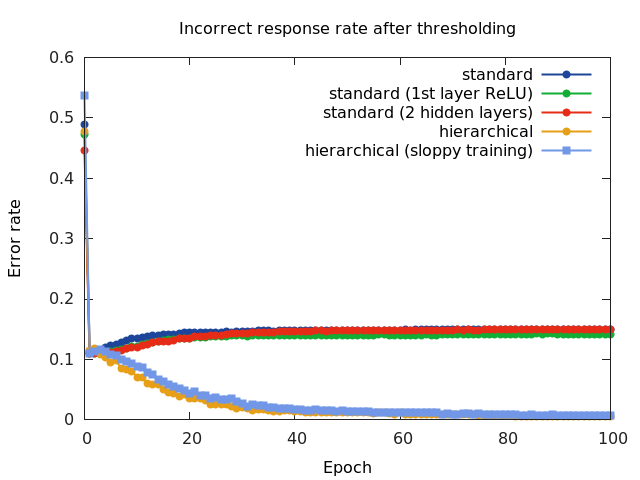
\includegraphics[width=0.65\textwidth]{abstract_figure.png}
    \caption{Error rates for $n = 64$, averaged across 100 trials}
    \label{abstract_figure}
\end{figure}

\end{document}
